\chapter{Introduction}
Over the last century, phones have changed from big and clumsy boxes that were mostly used to transfer simple spoken information over long distances into something different. Nowadays, mobile phones or smartphones are devices that allow us to navigate through big cities we have never been to before, translate conversations between people speaking different languages, find and recognize objects through the camera, and provide us with context.

Board games have likewise changed from the simplest ones, such as checkers, which can be played on any surface with a checkerboard pattern and rocks of different colors or shapes, into complex games that require players to study an entire book to play them correctly. An example of such a game would be Dungeons and Dragons and similar games. 

Having a device with a camera and hardware capable of analyzing images in our pockets could help solve problems with games that are too complex or just hard to learn. Applications that combine computer vision and board games ease the learning curve of games and shorten the time it takes for new players to grasp the basics of the game. These applications were called smart assistants by one of my predecessors who explored this topic. 

However, the main goal of this thesis is not to create a functional assistant application, but rather to create an end-to-end computer vision pipeline that will help develop these applications.

Computer Vision Inference Library for Board Games, or CV.ILIBG, is an Android library written in Kotlin, whose purpose is to provide an abstract layer for developers that will allow them to speed up the development of applications that use computer vision to detect board game objects. Furthermore, the library contains template functions for loading assets, storing user data, and other useful tools for repetitive tasks.

Part of this pipeline is also a desktop application written in Python, whose purpose is to import unlabeled and unordered data; in this case, images, label them, create synthetic data that will enhance the results of the final model, and lastly, use a deep neural network trainer to turn them into models that can be used for object detection in the Android library.


\chapter{Literature}

\section{Computer Vision}
\label{ComputerVision}
Computer vision is the ability of a machine to perform visual tasks of recognizing and processing image data \cite{computerVisionIBM}. To us humans, this is something we don't even think about. However, the process of recognizing that an object with orange color and sphere-like geometry is an orange is more complicated than we might think.

\subsection{Object detection}

Detecting objects inside an image has been a difficult task for computer vision researchers for a long time. In 2001, Viola \cite{viola} introduced a rapid object detection system capable of detecting facial features in real-time. In 2012, Krizhevsky \cite{krizhevsky} made a significant leap by introducing Deep Convolutional Neural Networks (hereafter referred to as DNN). This changed how object detection was performed, instead of handcrafting the features, it became possible to train a model on annotated data \cite{Xue2024ObjectDetection}. The AlexNet \cite{krizhevsky} laid the groundwork for future models and research.

The general object detection can be semantically grouped into categories of computer vision detection. \textbf{Image Classification} \cite{imageClassificationIBM} is the first and one of the easiest tasks. It classifies the image as a whole. \textbf{Object Detection} \cite{objectDetectionIBM} is a further expansion upon image classification, and instead of classifying the whole image, it returns a list of coordinates or regions that contain certain objects, along with the confidence score for these objects. These coordinates are usually in the form of rectangles and contain x and y coordinates along with the width and height. These are called bounding boxes.

The DNN is not a solution to object detection on its own. The DNN describes a family of neural networks that use deep learning to achieve object detection. These models differ in architecture and principles. The survey taken in 2024 \cite{objectDetectionSurver2024} explores the most popular models and their different versions. The article concludes that You Only Look Once (from now on, YOLO) is the most efficient model, as it achieves the best performance among the tested models. Another survey in 2025 reaches a similar conclusion, with YOLO dominating in performance even at the cost of lower precision.

\subsection{YOLO - You Only Look Once}
\label{yolo}
In 2016, a Redmon presented a new single shot model called YOLO \cite{Redmon_2016_CVPR}. Other approaches, like R-CNN, that search the image for possible bounding boxes and then run classifiers on those parts of the image, are also called two stage classifiers. YOLO uses a different approach. A single convolutional network predicts both bounding boxes and confidence scores for those bounding boxes in a single step. This approach makes YOLO fast in comparison with, up to that point in time, state-of-the art two stage models. It also provides more context, as the model sees the image as a whole, unlike R-CNN, which uses a sliding window that results in networks lacking context about the entire image.

\subsection{Ultralytics}
\label{Ultralytics}
Ultralytics is a company that provides tools for object detection, image segmentation, and other machine learning solutions. Their official site says that their aim is to make AI easy and accessible to individuals and businesses \cite{ultralyticsAbout}. This thesis uses Ultralytics's YOLO pretrained neural networks for object detection tasks. These pretrained models are further trained with the Ultralytics Python library to detect objects for a specific board game. This all in one solution allows for simplicity during the training of models that can be further exported into the more versatile Open Neural Network Exchange format (ONNX, see \ref{chosingInferenceEngine}).


\subsection{Transfer learning and pre-trained models}   
\label{pretrainedModels}
Training reliable neural networks is expensive, both in terms of time and computational power. However, training models on only a few hundred images might result in inefficient model accuracy. However, training on huge datasets such as the COCO dataset, which contains hundreds of thousands of labeled images, for hundreds of epochs would be nearly impossible for smaller developers who do not have access to powerful hardware focused on these tasks.

\textbf{Transfer learning} is a solution to this problem. This method allows developers to use the weights of neural networks that have been trained on these huge datasets and use these weights as a base for their model. By "freezing" the first \texttt{N} layers of the convolutional network and training only the last few layers, it is possible to utilize the knowledge that the original neural network learned \cite{transferLearning} \cite{pretrainedWeights}. For example, it is much easier to learn a new programming language if we already know at least one other programming language or have at least a basic understanding of how computers work.

\section{Data augmentation}
\label{dataAugmentation}
Deep neural networks, specifically convolutional neural networks, need data for training the models. It is generally accepted that larger datasets result in more accurate DNNs \cite{dataAugmentation2}. However, training sophisticated models with an insufficient amount of data might result in \textbf{overfitting} \cite{dataAugmentation1}. This phenomenon occurs when the training loss of the model declines with the number of epochs that the model was trained on; however, the validation loss is not declining but rising. Once these two values start diverging from one another, overfitting occurs.

\begin{figure}[hbt]
	\centering
	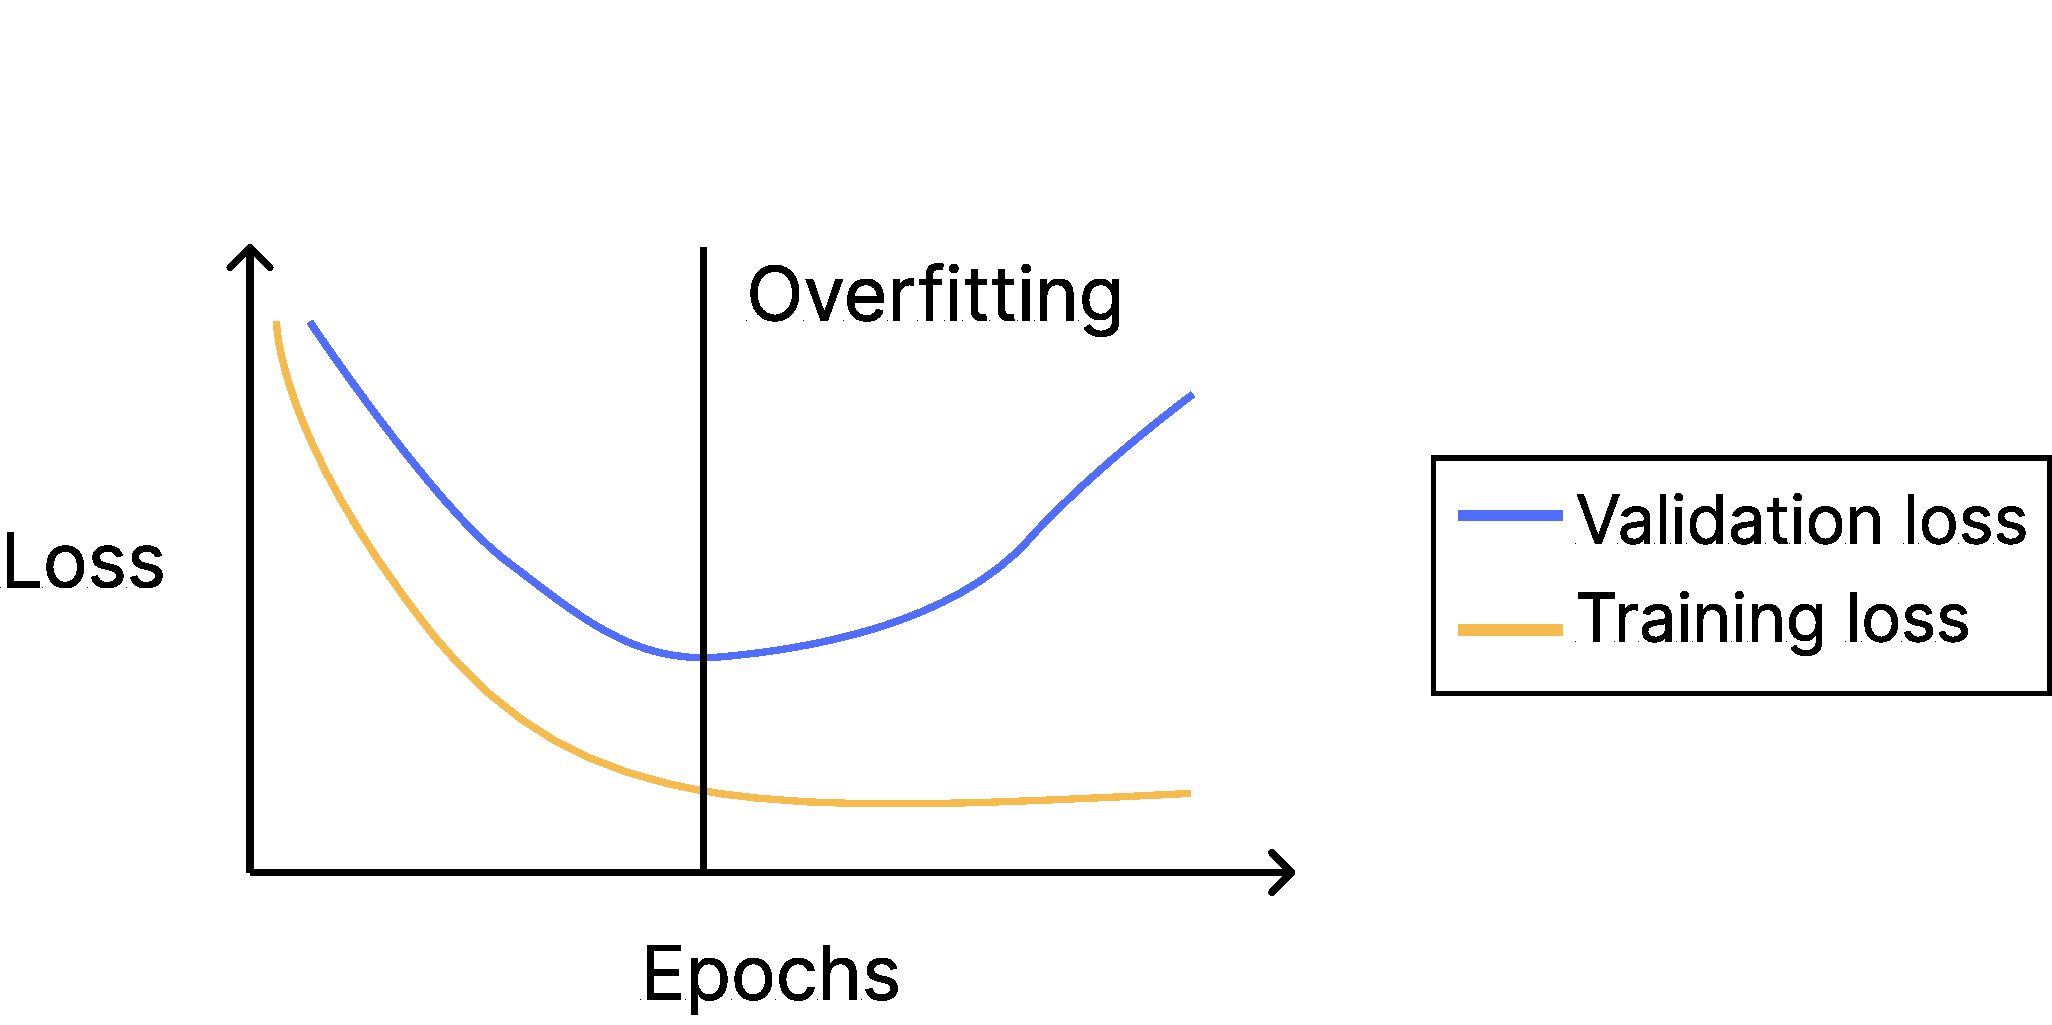
\includegraphics[width=0.6\textwidth]{obrazky-figures/overfitting.pdf}
	\caption[Overfitting illustrative graph]{An illustration of overfitting. Obtained from \cite{dataAugmentation1} and remade into PDF format for lossless scaling}
	\label{overfitting}
\end{figure}

Overfitting can be addressed by obtaining more training data; however, obtaining data for medical, niche, or generally difficult fields, for which producing more data is not viable. 

Data augmentation solves this problem by creating artificial/synthetic data. These can be created using traditional and deep learning/generative methods. This thesis focuses more on traditional methods; therefore, those will be the main part of the discussion.


% ===========================================================================================

% ===========================================================================================

\section{Previous works}


% ===========================================================================================

% ===========================================================================================

